\documentclass[11pt,a4paper]{article}

% =========================================================
% PACKAGES
% =========================================================
\usepackage[a4paper,margin=0.72in]{geometry}
\usepackage{enumitem}
\usepackage{titlesec}
\usepackage{hyperref}
\usepackage{tabularx}
\usepackage{array}
\usepackage{xcolor}
\usepackage{microtype}
\usepackage{setspace}
\usepackage{graphicx}

% =========================================================
% HYPERLINK SETTINGS
% =========================================================
\hypersetup{
    colorlinks=true,
    linkcolor=black,
    urlcolor=blue,
    citecolor=black
}

% =========================================================
% PAGE AND PARAGRAPH SETTINGS
% =========================================================
\setlength{\parindent}{0pt}
\setlength{\parskip}{0pt}
\setlength{\tabcolsep}{4pt}

\setlist[itemize]{
    leftmargin=1.4em,
    itemsep=1.5pt,
    topsep=2pt,
    parsep=0pt,
    partopsep=0pt
}

% =========================================================
% SECTION STYLE
% =========================================================
\titleformat{\section}
    {\large\bfseries}
    {}
    {0pt}
    {}
    [\vspace{-4pt}\rule{\textwidth}{0.5pt}]

\titlespacing{\section}
    {0pt}
    {10pt}
    {5pt}

% =========================================================
% CUSTOM COMMANDS
% =========================================================

\newcommand{\cvitem}[2]{
    \textbf{#1} & #2 \\[2pt]
}

\newcommand{\entry}[4]{
    \textbf{#1} \hfill \textit{#2}\\
    \textit{#3} \hfill #4
    \vspace{3pt}
}

\newcommand{\researchentry}[3]{
    \textbf{#1} \hfill \textit{#2}\\
    #3
    \vspace{4pt}
}

\usepackage{fontawesome5}
\usepackage{xcolor}
\usepackage{hyperref}

\definecolor{iconcolor}{RGB}{150,70,10}

\hypersetup{
    colorlinks=true,
    urlcolor=blue,
    linkcolor=blue
}

% =========================================================
% DOCUMENT
% =========================================================
\begin{document}

% =========================================================
% HEADER
% =========================================================

\noindent
\begin{minipage}[c]{\textwidth}
    \centering
    {\LARGE \textbf{Curriculum Vitae}}\\[0.4cm]
    {\Large \textbf{Rangan Chakrabarty}}
\end{minipage}

\vspace{-2.3cm}
\begin{flushright}
    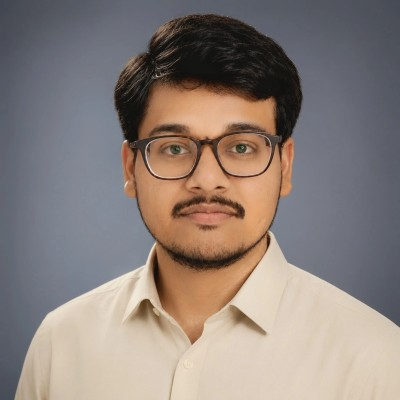
\includegraphics[width=2.8cm,height=3.5cm,keepaspectratio]{pic.jpg}
\end{flushright}

\vspace{0.1cm}
\begin{minipage}[t]{0.50\textwidth}
    \raggedright
    \small

    \faMapMarker* \hspace{3pt} Jadavpur University, Kolkata, West Bengal, India\\[-1pt]
    \faMapMarker* \hspace{3pt} Katwa, Purba Bardhaman, West Bengal, India

\end{minipage}
\hfill
\begin{minipage}[t]{0.46\textwidth}
    \raggedleft
    \small

    \faEnvelope \hspace{3pt}
    \href{mailto:ranganc.physics.ug@jadavpuruniversity.in}
    {ranganc.physics.ug@jadavpuruniversity.in}\\[-1pt]

    \faPhone \hspace{3pt}
    (+91) 8942957625\\[-1pt]

    \faLinkedin \hspace{3pt}
    \href{https://www.linkedin.com/in/reach2rcju/}{LinkedIn}
    \quad $\vert$ \quad
    \faResearchgate \hspace{3pt}
    \href{https://www.researchgate.net/profile/Rangan-Chakrabarty?ev=hdr_xprf}
    {ResearchGate}\\[-1pt]

    \faGlobe \hspace{3pt}
    \href{https://rangan269-ju.github.io/Personalwebsite/}{Personal website}

\end{minipage}


% =========================================================
% RESEARCH INTERESTS
% =========================================================

\section{Areas of Interest}

Quantum Information Theory, Quantum Communication


% =========================================================
% EDUCATION
% =========================================================

\section{Academic Credentials}

\entry
{Jadavpur University}
{2023 -- 2027}
{4-year B.Sc. (Hons. with Research) in Physics}
{Kolkata, India}

\begin{itemize}
    \item Cumulative Percentage till 6th Sem: \textbf{77.19\%} \hspace{5pt}
\end{itemize}

\vspace{2pt}

\entry
{Katwa Kashiram Das Institution}
{2020}
{Higher Secondary (HS) Examination, WBCHSE}
{WB, India}

\begin{itemize}
    \item Percentage: \textbf{85.8\%} \hspace{5pt} Grade: \textbf{A+}
\end{itemize}

\vspace{2pt}

\entry
{Katwa Kashiram Das Institution}
{2018}
{Madhyamik Examination, WBBSE}
{WB, India}

\begin{itemize}
    \item Percentage: \textbf{86.71\%} \hspace{5pt} Grade: \textbf{A+}
\end{itemize}


% =========================================================
% SCHOLASTIC ACHIEVEMENTS
% =========================================================

\section{Scholastic Achievements}

\begin{itemize}
    \item \textbf{HRI Visiting Students Research Program (VSP), 2026-27}
    -- Selected / 
    \item \textbf{IISER Bhopal Summer Internship Program (SIP), 2026}
    -- Selected / \href{https://drive.google.com/file/d/19KI8KwJgoWlNMxhyr6JmX6We5U1eYqXy/view}{Offer Letter}.

    \item \textbf{GRISHMA Summer Research Program, IIT Kharagpur}
    -- Selected (not joined due to overlapping schedule) / \href{https://drive.google.com/file/d/15TsCT1BaY7Ln1zuf8dIu2j2J3oRW39ya/view}{Offer Letter}.

    \item \textbf{IASc--INSA--NASI Summer Research Fellowship Program,
    2025}, India -- Selected / \href{https://drive.google.com/file/d/1c7MNgjkSZGNMjPqBJrUiEm1o9r3ER1DS/view}{Offer Letter}.

    \item \textbf{Silver Honour}, IAAC, Germany, 2024 / \href{https://drive.google.com/file/d/1Qcdn53l4dRz0xNyGqWUqF-QKqerZJ1hD/view}{Certificate}.

\end{itemize}


% =========================================================
% RESEARCH EXPERIENCE
% =========================================================

\section{Research Experience}

\entry
{Harish-Chandra Research Institute, Prayagraj}
{Oct 2026 --}
{Visitng Student}
{Prayagraj, UP, India}\\
\textbf{Supervisor:} Prof. Ujjwal Sen, Professor \& Director, HRI


\vspace{0.5cm}

\entry
{IISER Kolkata \& SOADU, Bhubneswar}
{Sept 2026 --}
{Undergraduate Research Assistant}
{Kolkata, WB, India}\\
\textbf{Supervisor:} Prof. Prasanta K. Panigrahi, Emeritus Professor and Former Director, IISER Kolkata; Director, CQST, SOADU

\vspace{0.5cm}

\entry
{Indian Institute of Science Education \& Research, Bhopal}
{May 2026 -- August 2026}
{Summer Internship Trainee}
{Bhopal, MP, India}

\textbf{Project Title:} Quantum Dense Coding Using Bipartite and Multipartite Entangled States Over Noiseless and Noisy Quantum Channels: An IBM Quantum Experience. \href{https://drive.google.com/file/d/1J3n-vC0oDD9sEbbBHkWpspZd-wM6JGFF/view}{Project Report}\\
\textbf{Supervisor:} Prof. Kuntal Roy, EECS Department, IISER Bhopal

\vspace{0.5cm}

\entry
{Bose Institute, Kolkata}
{July 2025 -- September 2025}
{Summer Research Fellow}
{Kolkata, WB, India}

\textbf{Project Title:} Quantum Algorithms: Detailed Study, Experimental Implementations and Fault Diagnosis of Quantum Logic Gates. \href{https://drive.google.com/file/d/1E1iEWA_XGIpx8ue8O8EmcbC7oqrU1EMY/view}{Project Report} / \href{https://drive.google.com/file/d/1NBCb0vpF9wkKBZtGyaOdMJWQPaDDwR7G/view}{Certificate}\\
\textbf{Supervisor:} Prof. Somshubhro Bandyopadhyay, Department of Physical Sciences, Bose Institute\\
\textit{Jointly Sponsored by IASc--INSA--NASI, SRFP 2025}


% =========================================================
% SCHOLARLY WORK
% =========================================================

\section{Scholarly Work}

\subsection*{Publications}

\begin{enumerate}[leftmargin=1.6em,label={[\arabic*]}]

    \item \textbf{Superdense Coding Protocol in Maximally and
    Non-maximally Entangled Bell State: An Experimental Realisation.}

    Published in the \textit{Abstract Book: Scientific Innovation and Skill Development for Societal Advancement}, Innovation \& Skill Development Research Centre (ISDRC), Jadavpur University,
    India, 2026. \href{https://drive.google.com/file/d/1ToPfW1x9e7QYZ5J9rGE3fAvibrJyEWTS/view}{Abstract}

    \item \textbf{Ancilla-Entangled Modified Qutrit Deutsch--Jozsa (DJ) Algorithm for Useful Discrimination Between Function Types of an Odd-Level Qudit System.}

    Published in the \textit{Abstract Book: Scientific Innovation
    and Skill Development for Societal Advancement}, ISBN:
    978-81-987857-6-3, Innovation \& Skill Development Research Centre (ISDRC), Jadavpur University, India, 2025. \href{https://drive.google.com/file/d/1ACMXFrVa7RHp0wzm-JgYlG7j_JYHoosi/view}{Abstract}

\end{enumerate}


% =========================================================
% PRESENTATIONS
% =========================================================

\subsection*{Presentations}

\begin{itemize}

    \item \textbf{Poster Presentation:} ``Superdense Coding Protocol in Maximally and Non-maximally Entangled Bell State: An Experimental Realisation.''\\
Presented at \textit{Presision-2026}, Presidency University, Kolkata, and \textit{SISDSA-2026}, Jadavpur University (Won $2^{nd}$ prize). \href{https://drive.google.com/file/d/1eJ5AMMzWMnt3Mb0F7u2ODuxFsIbAxwHX/view}{Poster}

    \item \textbf{Oral Presentation:} ``Quantum Algorithms:
    Detailed Study, Experimental Implementations and Fault Diagnosis of Quantum Logic Gates.''\\
    Presented at Bose Institute, Kolkata, and the Department of Physics, Jadavpur University, 2025.

\end{itemize}


% =========================================================
% WORKSHOPS AND COURSES
% =========================================================

\section{Academic Achievements}
\subsection*{Workshops, Schools and Courses}

\begin{itemize}

    \item \textbf{CERN--MPQ--UIBK School on Quantum Simulation of Fundamental Physics}, 17 August -- 4 September 2026.
    \item \textbf{Introduction to Quantum Computing in Fluid Dynamics (STO-AVT-377)}, Von Karman Institute for Fluid Dynamics, Belgium, 6--10 July 2026.
    \item \textbf{International Workshop on Nano-photonics using Structured Light}, IISER Kolkata and University at Buffalo, SPARC, 7 March 2026. \href{https://drive.google.com/file/d/1uOrKydeN2anYDa1a1ZPAUAngxF0hprEo/view}{Certificate}
    \item \textbf{Workshop on Quantum Computing and Quantum Key Distribution (QKD)}, IIT Delhi, 27 February -- 1 March 2026. \href{https://drive.google.com/file/d/1TL8kjZkPKYqeoUk7mt9nnWZ4h8DkPc3u/view}{Certificate}
    \item \textbf{Familiarisation Workshop on Quantum Computing}, Foundation for QC Innovations, IISc, India, 2026. \href{https://drive.google.com/file/d/1WVQtCkAq4JrkASNk-tq-9vaVKKrF60OO/view}{Certificate}
    \item \textbf{Workshop on Quantum Computing and Algorithms, IIT Kharagpur, India}, 31 January and 1 February 2026,  \href{https://drive.google.com/file/d/1LOt6r0R2hUTHvXDmhl740sPYz4gOO94r/view?usp=drive_link}{Certificate}
    \item \textbf{Summer School on Correlated Quantum Materials \& Solid-State Quantum Systems 2025}, Julius-Maximilians-Universität Würzburg, Germany, 15--19 September 2025.
    \item \textbf{INUP-i2i online familiarization workshop on nanofabrication \& characterisation- IIT KGP}, 2025, \href{https://drive.google.com/file/d/1IqakSE80kBtRvirf6UG0MSezLZISpIji/view?usp=drive_link}{Certificate}
    \item \textbf{QuCAM: Quantum Computing -- Circuits, Algorithms,\& Machine Learning Workshop}, NIT Rourkela, India, 2025.
    \item \textbf{Introductory Course on Quantum Computing},
    IISER Pune, India, 2024--25. \href{https://drive.google.com/file/d/1sgIMb-mWTsk6QFnRIglUeTgSHb6mNWAt/view}{Certificate}

    \item \textbf{AI Winter School}, Centre for Fundamental Physics of the Universe, Brown University, USA, 2025. \href{https://drive.google.com/file/d/1ORo3sxO7IakUHW4bqKJBtPJqxbwnikIp/view}{Certificate}
    \item \textbf{Winter School on Semiconductor Technology},
    Centre for Nano Science and Engineering (CeNSE), IISc, India, 2024. \href{https://drive.google.com/file/d/1SZiUrxu9o2Ie2XDfJy9m4O4ctlaH4kSJ/view}{Certificate}

    \item \textbf{Workshop on Classical and Quantum Machine Learning for Condensed Matter Physics}, ICTP, Italy, 2024. \href{https://drive.google.com/file/d/1ERSvCGcr1wE6zF4m50vy1_SHyIbEuXgu/view}{Invitation Letter}

\end{itemize}
% =========================================================
% TECHNICAL SKILLS
% =========================================================

\section{Technical Skills}

\begin{tabularx}{\textwidth}{@{}>{\bfseries}p{3.0cm}X@{}}

Programming Languages &
Python, Fortran-95 \\[3pt]

Quantum Computing &
Qiskit SDK, IBM QE, IonQ Cloud \\[3pt]

Scientific Computing &
NumPy, SciPy, Matplotlib, Gnuplot \\[3pt]

Scientific Skills &
Scientific writing, literature review, numerical analysis \\[3pt]

Typesetting &
LaTeX \\

\end{tabularx}


% =========================================================
% LANGUAGES
% =========================================================

\section{Languages}

\begin{tabularx}{\textwidth}{@{}>{\bfseries}p{3.0cm}X@{}}

English & Reading, Writing, Speaking \\[2pt]

Bengali & Mother Tongue \\[2pt]

Hindi & Reading, Speaking \\

\end{tabularx}


% =========================================================
% LEADERSHIP AND ACADEMIC ACTIVITIES
% =========================================================

\section{Leadership and Academic Activities}

\begin{itemize}

    \item \textbf{Club Head, Quantum Physics Club},
    Jadavpur University.

    \item \textbf{Photography Club},
    Jadavpur University.

    \item \textbf{Founding Member, Innovation and Skill Development
    Research Centre (ISDRC)}, Jadavpur University.

\end{itemize}


% =========================================================
% REFERENCES
% =========================================================

\section{References}
Prof. Nabin Baran Manik, Dept. of Physics, JU\\
Prof. Ajay Kumar Ghosh, Dept. of Physics, JU\\


\vfill

\begin{center}
\small
Last updated on \number\day/\number\month/\number\year
\end{center}

\end{document}
```
